\chapter{Kết quả thực nghiệm và đánh giá}
\section{Tính toàn vẹn dữ liệu và kết quả tổng quát}
Thực nghiệm chính thức ngày 12/11/2026 bắt đầu lúc 16:32:58 và kết thúc lúc 16:42:26 (UTC+7), khoảng 9 phút 28 giây, trên commit \texttt{ab588fb}. Chín phiên đều có đúng 275 lượt: 25 warm-up và 250 mẫu chính thức; tổng 2250 mẫu được nhận, không lỗi, timeout hoặc mẫu bị loại. Requested và actual threads khớp tại 1/2/4/8. Analyzer kiểm hash, đầy đủ cấu hình, warm-up và chỉ số lần lặp trước khi tổng hợp. Bản sao ổ D được đối chiếu từng file.

Giám sát ghi nguồn AC trong toàn bộ phiên; RAM trống thấp nhất 11\,135\,807\,488 byte (khoảng 10,37 GiB). Tải CPU nền đo một giây trước mỗi phiên nằm trong khoảng 1,30--19,01\%; đây không phải tải nền đo liên tục trong BFS. Không có số đo nhiệt độ để khẳng định máy không throttling. Toàn bộ bảng/biểu đồ dùng raw thật, không dùng timing CI hoặc fixture unit test.

\textbf{Không có cấu hình OpenMP nào nhanh hơn Serial trên ma trận này.} Trong 216 cấu hình OpenMP, speedup lớn nhất là 0,2914 ở Optimized một luồng/static/grid512 nguồn 0 (5,814 ms so Serial 1,6942 ms). Khi xét team từ hai luồng, scaling so OpenMP một luồng lớn nhất cũng chỉ 0,7536 ở Basic hai luồng/static/star một triệu đỉnh. Đây là kết quả của phép đo lời gọi độc lập trên tập dữ liệu đã chốt, không phải kết luận mọi BFS song song đều chậm.

\begin{table}[htbp]\centering\small
\caption{Ba đồ thị lớn, nguồn 0, static, actual 8; median theo ms, speedup so Serial, 10 mẫu/cấu hình.}\label{tab:headline}
\begin{tabular}{lrrrrr}\toprule
Đồ thị & Serial & Basic8 & Opt8 & $S_{B,8}$ & $S_{O,8}$ \\\midrule
Path8192 & 0,05185 & 922,0907 & 1562,0243 & 0,00005623 & 0,00003319 \\
Star1000000 & 3,1294 & 26,4158 & 26,4872 & 0,1185 & 0,1181 \\
Grid512 & 1,6942 & 112,6744 & 179,7294 & 0,01504 & 0,009426 \\\bottomrule
\end{tabular}\end{table}

\section{Bảng thống kê theo cấu hình}
Các bảng sau trình bày mọi mức luồng với static: Serial baseline, median, IQR, speedup, efficiency theo team thực và scaling so OpenMP một luồng. Không chọn schedule thắng để thay ma trận. Tệp đi kèm \texttt{results/experiment-20261112/summary.csv} chứa đầy đủ 225 dòng với cả static/dynamic/guided, min, max, $Q_1$ và $Q_3$. Serial là một baseline cho mỗi đồ thị/nguồn. Số hiển thị được làm tròn; phép tính và tệp máy đọc giữ độ chính xác gốc.
\begin{table}[htbp]
\centering\small
\caption[path2048-s0: thống kê static]{path2048-s0: median và IQR theo ms, static; 10 mẫu/cấu hình. $S$ so Serial, $E$ theo team thực, $C$ so OpenMP một luồng.}
\label{tab:path2048-s0}
\begin{tabular}{lrrrrrr}
\toprule
Phiên bản & $p$ & Median & IQR & $S$ & $E$ (\%) & $C$ \\
\midrule
Serial & 1 & 0,0097 & 0 & 1 & 100 & -- \\
Basic & 1 & 0,2198 & 0,0123 & 0,04414 & 4,414 & 1 \\
Basic & 2 & 59,01 & 2,527 & 0,0001644 & 0,008219 & 0,003724 \\
Basic & 4 & 123,4 & 3,985 & $7,858\times10^{-5}$ & 0,001965 & 0,00178 \\
Basic & 8 & 229,4 & 16,84 & $4,228\times10^{-5}$ & 0,0005284 & 0,0009577 \\
Optimized & 1 & 0,2786 & 0,005475 & 0,03481 & 3,481 & 1 \\
Optimized & 2 & 97,08 & 2,486 & $9,991\times10^{-5}$ & 0,004996 & 0,00287 \\
Optimized & 4 & 204,8 & 5,98 & $4,737\times10^{-5}$ & 0,001184 & 0,001361 \\
Optimized & 8 & 390 & 20,15 & $2,487\times10^{-5}$ & 0,0003109 & 0,0007146 \\
\bottomrule
\end{tabular}
\end{table}

\begin{table}[htbp]
\centering\small
\caption[path8192-s0: thống kê static]{path8192-s0: median và IQR theo ms, static; 10 mẫu/cấu hình. $S$ so Serial, $E$ theo team thực, $C$ so OpenMP một luồng.}
\label{tab:path8192-s0}
\begin{tabular}{lrrrrrr}
\toprule
Phiên bản & $p$ & Median & IQR & $S$ & $E$ (\%) & $C$ \\
\midrule
Serial & 1 & 0,05185 & 0,006975 & 1 & 100 & -- \\
Basic & 1 & 0,6653 & 0,01063 & 0,07793 & 7,793 & 1 \\
Basic & 2 & 238,1 & 10,31 & 0,0002178 & 0,01089 & 0,002794 \\
Basic & 4 & 493,6 & 15,19 & 0,0001051 & 0,002626 & 0,001348 \\
Basic & 8 & 922,1 & 45,46 & $5,623\times10^{-5}$ & 0,0007029 & 0,0007215 \\
Optimized & 1 & 0,8969 & 0,01422 & 0,05781 & 5,781 & 1 \\
Optimized & 2 & 392 & 4,749 & 0,0001323 & 0,006613 & 0,002288 \\
Optimized & 4 & 831,2 & 16,72 & $6,238\times10^{-5}$ & 0,001559 & 0,001079 \\
Optimized & 8 & 1562 & 76,62 & $3,319\times10^{-5}$ & 0,0004149 & 0,0005742 \\
\bottomrule
\end{tabular}
\end{table}

\begin{table}[htbp]
\centering\small
\caption[path8192-s4096: thống kê static]{path8192-s4096: median và IQR theo ms, static; 10 mẫu/cấu hình. $S$ so Serial, $E$ theo team thực, $C$ so OpenMP một luồng.}
\label{tab:path8192-s4096}
\begin{tabular}{lrrrrrr}
\toprule
Phiên bản & $p$ & Median & IQR & $S$ & $E$ (\%) & $C$ \\
\midrule
Serial & 1 & 0,0372 & 0,0034 & 1 & 100 & -- \\
Basic & 1 & 0,4464 & 0,0103 & 0,08332 & 8,332 & 1 \\
Basic & 2 & 116,8 & 4,529 & 0,0003186 & 0,01593 & 0,003824 \\
Basic & 4 & 243,1 & 6,511 & 0,0001531 & 0,003826 & 0,001837 \\
Basic & 8 & 468,4 & 18,49 & $7,941\times10^{-5}$ & 0,0009926 & 0,000953 \\
Optimized & 1 & 0,5499 & 0,008075 & 0,06765 & 6,765 & 1 \\
Optimized & 2 & 194,3 & 3,152 & 0,0001915 & 0,009575 & 0,002831 \\
Optimized & 4 & 409,8 & 14,78 & $9,078\times10^{-5}$ & 0,00227 & 0,001342 \\
Optimized & 8 & 767 & 42,57 & $4,85\times10^{-5}$ & 0,0006062 & 0,0007169 \\
\bottomrule
\end{tabular}
\end{table}

\begin{table}[htbp]
\centering\small
\caption[star100000-s0: thống kê static]{star100000-s0: median và IQR theo ms, static; 10 mẫu/cấu hình. $S$ so Serial, $E$ theo team thực, $C$ so OpenMP một luồng.}
\label{tab:star100000-s0}
\begin{tabular}{lrrrrrr}
\toprule
Phiên bản & $p$ & Median & IQR & $S$ & $E$ (\%) & $C$ \\
\midrule
Serial & 1 & 0,2825 & 0,1892 & 1 & 100 & -- \\
Basic & 1 & 1,811 & 0,1583 & 0,156 & 15,6 & 1 \\
Basic & 2 & 3,459 & 0,5684 & 0,08167 & 4,084 & 0,5236 \\
Basic & 4 & 3,872 & 1,072 & 0,07296 & 1,824 & 0,4678 \\
Basic & 8 & 4,332 & 0,9949 & 0,06521 & 0,8151 & 0,4181 \\
Optimized & 1 & 1,529 & 0,1227 & 0,1848 & 18,48 & 1 \\
Optimized & 2 & 3,089 & 0,4858 & 0,09145 & 4,572 & 0,4949 \\
Optimized & 4 & 3,681 & 0,5019 & 0,07675 & 1,919 & 0,4154 \\
Optimized & 8 & 4,386 & 0,3927 & 0,06441 & 0,8051 & 0,3486 \\
\bottomrule
\end{tabular}
\end{table}

\begin{table}[htbp]
\centering\small
\caption[star1000000-s0: thống kê static]{star1000000-s0: median và IQR theo ms, static; 10 mẫu/cấu hình. $S$ so Serial, $E$ theo team thực, $C$ so OpenMP một luồng.}
\label{tab:star1000000-s0}
\begin{tabular}{lrrrrrr}
\toprule
Phiên bản & $p$ & Median & IQR & $S$ & $E$ (\%) & $C$ \\
\midrule
Serial & 1 & 3,129 & 0,1779 & 1 & 100 & -- \\
Basic & 1 & 17,68 & 0,7979 & 0,177 & 17,7 & 1 \\
Basic & 2 & 23,46 & 1,176 & 0,1334 & 6,67 & 0,7536 \\
Basic & 4 & 25,23 & 1,81 & 0,124 & 3,101 & 0,7007 \\
Basic & 8 & 26,42 & 1,165 & 0,1185 & 1,481 & 0,6693 \\
Optimized & 1 & 15,44 & 0,6806 & 0,2027 & 20,27 & 1 \\
Optimized & 2 & 23,23 & 1,789 & 0,1347 & 6,735 & 0,6645 \\
Optimized & 4 & 23,03 & 1,533 & 0,1359 & 3,397 & 0,6702 \\
Optimized & 8 & 26,49 & 2,311 & 0,1181 & 1,477 & 0,5828 \\
\bottomrule
\end{tabular}
\end{table}

\begin{table}[htbp]
\centering\small
\caption[star1000000-s1: thống kê static]{star1000000-s1: median và IQR theo ms, static; 10 mẫu/cấu hình. $S$ so Serial, $E$ theo team thực, $C$ so OpenMP một luồng.}
\label{tab:star1000000-s1}
\begin{tabular}{lrrrrrr}
\toprule
Phiên bản & $p$ & Median & IQR & $S$ & $E$ (\%) & $C$ \\
\midrule
Serial & 1 & 3,189 & 0,4142 & 1 & 100 & -- \\
Basic & 1 & 17,08 & 0,3277 & 0,1867 & 18,67 & 1 \\
Basic & 2 & 23,34 & 1,094 & 0,1367 & 6,833 & 0,7319 \\
Basic & 4 & 23,91 & 1,421 & 0,1334 & 3,334 & 0,7142 \\
Basic & 8 & 26,27 & 1,562 & 0,1214 & 1,517 & 0,6501 \\
Optimized & 1 & 15,51 & 0,9614 & 0,2056 & 20,56 & 1 \\
Optimized & 2 & 24,04 & 2,199 & 0,1326 & 6,632 & 0,645 \\
Optimized & 4 & 23,76 & 0,859 & 0,1342 & 3,355 & 0,6526 \\
Optimized & 8 & 25,63 & 1,863 & 0,1244 & 1,555 & 0,605 \\
\bottomrule
\end{tabular}
\end{table}

\begin{table}[htbp]
\centering\small
\caption[grid128-s0: thống kê static]{grid128-s0: median và IQR theo ms, static; 10 mẫu/cấu hình. $S$ so Serial, $E$ theo team thực, $C$ so OpenMP một luồng.}
\label{tab:grid128-s0}
\begin{tabular}{lrrrrrr}
\toprule
Phiên bản & $p$ & Median & IQR & $S$ & $E$ (\%) & $C$ \\
\midrule
Serial & 1 & 0,0912 & 0,0241 & 1 & 100 & -- \\
Basic & 1 & 0,5634 & 0,02492 & 0,1619 & 16,19 & 1 \\
Basic & 2 & 8,678 & 0,4216 & 0,01051 & 0,5255 & 0,06492 \\
Basic & 4 & 16,01 & 0,7455 & 0,005697 & 0,1424 & 0,03519 \\
Basic & 8 & 30,53 & 2,488 & 0,002987 & 0,03734 & 0,01846 \\
Optimized & 1 & 0,4789 & 0,01635 & 0,1904 & 19,04 & 1 \\
Optimized & 2 & 13,25 & 0,1796 & 0,006884 & 0,3442 & 0,03615 \\
Optimized & 4 & 26,43 & 0,8346 & 0,003451 & 0,08627 & 0,01812 \\
Optimized & 8 & 49,01 & 4,316 & 0,001861 & 0,02326 & 0,009773 \\
\bottomrule
\end{tabular}
\end{table}

\begin{table}[htbp]
\centering\small
\caption[grid512-s0: thống kê static]{grid512-s0: median và IQR theo ms, static; 10 mẫu/cấu hình. $S$ so Serial, $E$ theo team thực, $C$ so OpenMP một luồng.}
\label{tab:grid512-s0}
\begin{tabular}{lrrrrrr}
\toprule
Phiên bản & $p$ & Median & IQR & $S$ & $E$ (\%) & $C$ \\
\midrule
Serial & 1 & 1,694 & 0,3032 & 1 & 100 & -- \\
Basic & 1 & 7,043 & 0,5137 & 0,2405 & 24,05 & 1 \\
Basic & 2 & 37,73 & 2,058 & 0,04491 & 2,245 & 0,1867 \\
Basic & 4 & 63,98 & 3,206 & 0,02648 & 0,662 & 0,1101 \\
Basic & 8 & 112,7 & 8,654 & 0,01504 & 0,188 & 0,06251 \\
Optimized & 1 & 5,814 & 0,5139 & 0,2914 & 29,14 & 1 \\
Optimized & 2 & 52,54 & 4,019 & 0,03224 & 1,612 & 0,1106 \\
Optimized & 4 & 92,22 & 3,916 & 0,01837 & 0,4593 & 0,06305 \\
Optimized & 8 & 179,7 & 3,178 & 0,009426 & 0,1178 & 0,03235 \\
\bottomrule
\end{tabular}
\end{table}

\begin{table}[htbp]
\centering\small
\caption[grid512-s131328: thống kê static]{grid512-s131328: median và IQR theo ms, static; 10 mẫu/cấu hình. $S$ so Serial, $E$ theo team thực, $C$ so OpenMP một luồng.}
\label{tab:grid512-s131328}
\begin{tabular}{lrrrrrr}
\toprule
Phiên bản & $p$ & Median & IQR & $S$ & $E$ (\%) & $C$ \\
\midrule
Serial & 1 & 1,871 & 0,2011 & 1 & 100 & -- \\
Basic & 1 & 7,302 & 0,1272 & 0,2563 & 25,63 & 1 \\
Basic & 2 & 27,8 & 1,454 & 0,0673 & 3,365 & 0,2626 \\
Basic & 4 & 39,91 & 1,358 & 0,04688 & 1,172 & 0,1829 \\
Basic & 8 & 62,39 & 2,516 & 0,02999 & 0,3749 & 0,117 \\
Optimized & 1 & 6,68 & 0,6215 & 0,2801 & 28,01 & 1 \\
Optimized & 2 & 30,81 & 2,338 & 0,06072 & 3,036 & 0,2168 \\
Optimized & 4 & 52,66 & 1,867 & 0,03553 & 0,8883 & 0,1269 \\
Optimized & 8 & 92,55 & 2,286 & 0,02022 & 0,2527 & 0,07218 \\
\bottomrule
\end{tabular}
\end{table}

\clearpage

\section{Path: giới hạn của frontier hẹp}
Với nguồn 0, tăng path từ 2048 lên 8192 đỉnh (gấp4) làm median Serial tăng từ 0,0097 lên 0,05185 ms; Basic8/static từ 229,45 lên 922,09 ms, gần gấp4. Optimized 8/static từ 389,96 lên 1562,02 ms. Frontier chỉ có một đỉnh mỗi mức, nên tăng team không cung cấp thêm đỉnh cùng tầng để chia. Chi phí đồng bộ theo hàng nghìn mức phù hợp với xu hướng này; timer tổng chưa định lượng riêng barrier.

Basic một luồng/static mất0,6653 ms ở path8192, khoảng 12,8 lần Serial; actual 8 mất922,09 ms. Optimized 8 chậm hơn Basic8 khoảng 1,694 lần. Không thể giải thích toàn bộ chênh lệch chỉ bằng khởi tạo team một lần: tổ chức frontier/visited, lịch trình và đồng bộ lặp theo mức cũng có thể góp phần, cần profiling để tách riêng.

Đổi nguồn từ 0 sang 4096 giảm khoảng cách lớn nhất từ 8191 xuống4096. Basic8/static còn 468,45 ms (giảm 49,2\%), Optimized còn 767,02 ms (giảm 50,9\%). Quan sát phù hợp số mức giảm, nhưng hai nguồn chạy ở phiên riêng nên còn sai lệch thời điểm/tải nền. Cả hai vẫn chậm hơn Serial. Hình~\ref{fig:path-runtime}--\ref{fig:path-schedule} trình bày toàn bộ schedule và team.

\begin{figure}[p]\centering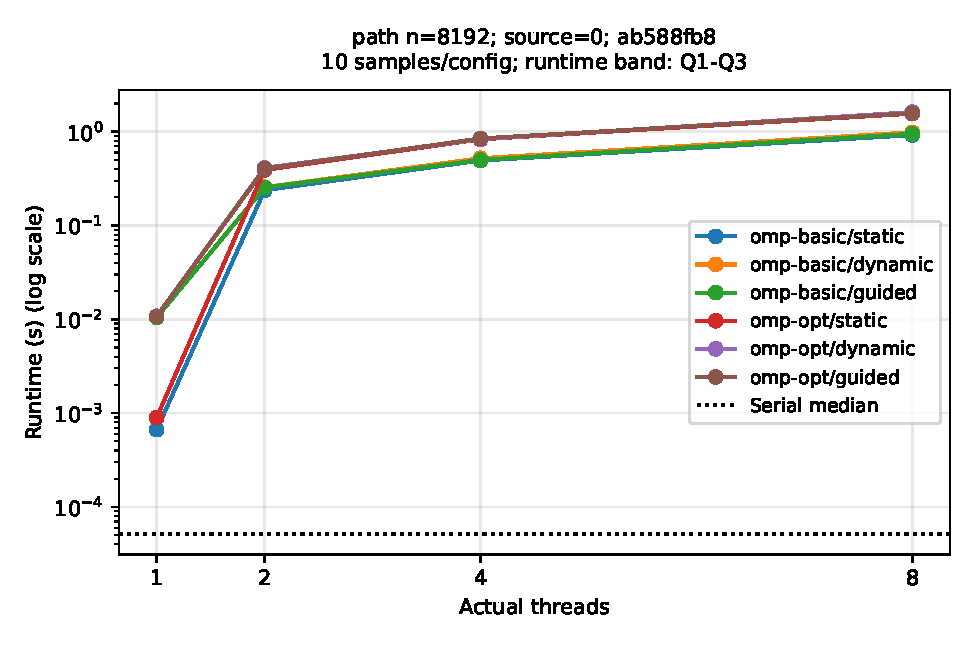
\includegraphics[width=.94\textwidth]{figures/experiment-20261112/path8192-s0/median.pdf}
\caption[Path8192: thời gian]{Path8192, nguồn 0, ab588fb: median và dải $Q_1$--$Q_3$, 10 mẫu/cấu hình; trục thời gian log để thấy cả Serial.}\label{fig:path-runtime}\end{figure}
\begin{figure}[p]\centering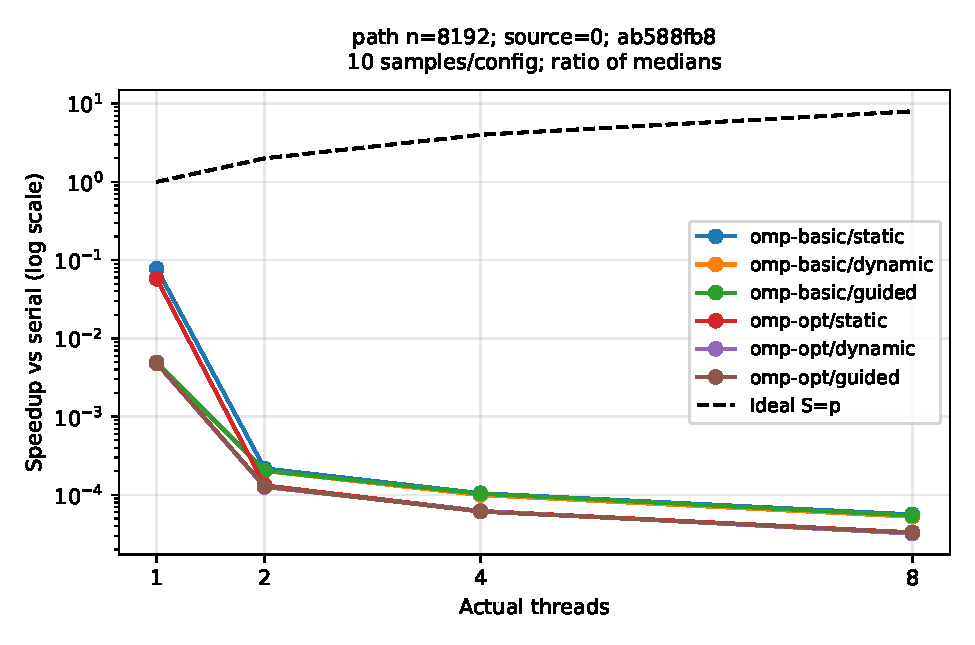
\includegraphics[width=.94\textwidth]{figures/experiment-20261112/path8192-s0/speedup.pdf}
\caption[Path8192: speedup]{Path8192, nguồn 0: speedup so Serial trên trục log; $S=p$ là mốc lý tưởng, không phải số đo.}\label{fig:path-speedup}\end{figure}
\begin{figure}[p]\centering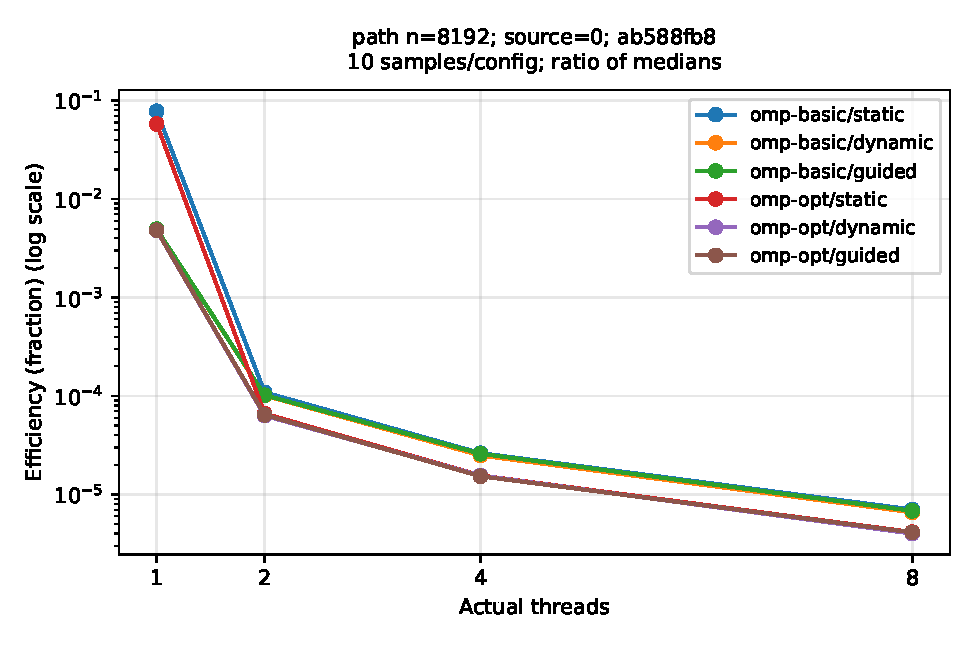
\includegraphics[width=.94\textwidth]{figures/experiment-20261112/path8192-s0/efficiency.pdf}
\caption[Path8192: efficiency]{Path8192, nguồn 0: efficiency $S/p$ theo team thực, 10 mẫu/cấu hình, commit ab588fb.}\label{fig:path-efficiency}\end{figure}
\begin{figure}[p]\centering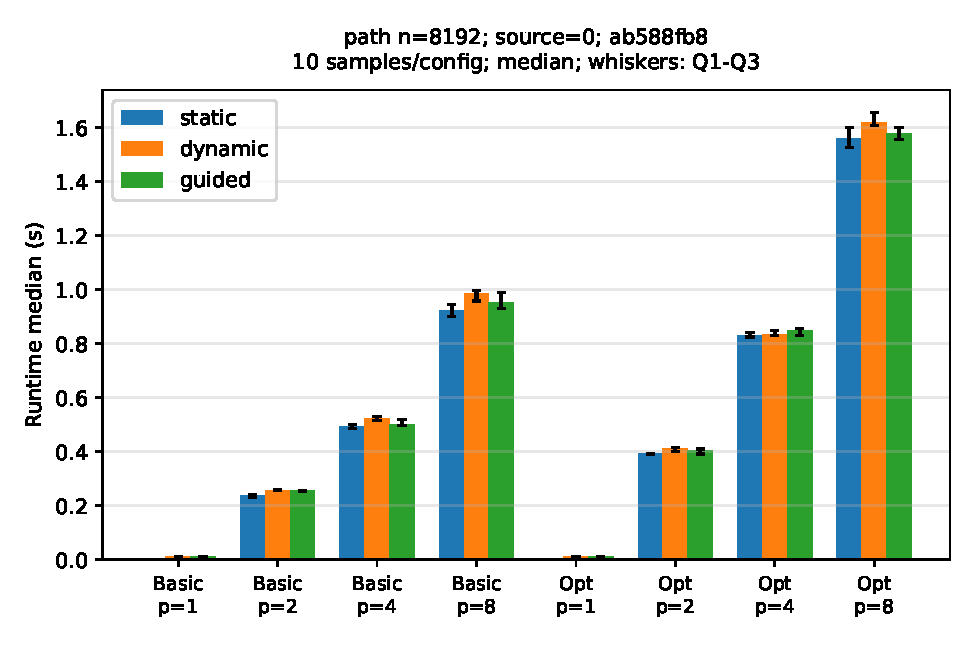
\includegraphics[width=.94\textwidth]{figures/experiment-20261112/path8192-s0/scheduling.pdf}
\caption[Path8192: scheduling]{Path8192, nguồn 0: scheduling trong cùng thuật toán/team; cột là median, thanh sai số là $Q_1$--$Q_3$.}\label{fig:path-schedule}\end{figure}
\clearpage

\section{Star: bậc lệch và chi phí lập lịch}
Star một triệu đỉnh có Serial median 3,1294 ms. Static/actual 8 cho Basic26,4158 ms và Optimized 26,4872 ms; speedup khoảng 0,118, efficiency khoảng 1,48\%. Hai median chênh0,0714 ms, nhỏ hơn IQR của mỗi bản (1,1649 và 2,3114 ms); chưa đủ cơ sở gọi Optimized tốt hơn. Ở bốn luồng/static, Optimized 23,0336 ms thấp hơn Basic25,2312 ms khoảng 8,7\%, nhưng lợi ích không nhất quán qua số luồng và vẫn chậm hơn Serial.

Đỉnh tâm có bậc999999 nhưng chỉ do một lần lặp frontier xử lý; vòng láng giềng trong một đỉnh không được chia cho nhiều luồng. Frontier sau đó rộng nhưng mỗi lá chỉ có một cung về tâm đã thăm. Nhiều đỉnh không đồng nghĩa nhiều công việc hữu ích cân bằng ở mọi mức; bỏ bộ đếm frontier chung chưa đủ bảo đảm tăng tốc.

Ở actual 8, dynamic làm Basic tăng từ 26,4158 lên 98,8135 ms (3,74 lần), Optimized từ 26,4872 lên 101,2997 ms (3,82 lần). Guided là 27,2610 và 26,1920 ms, gần static hơn. Điều này phù hợp giả thuyết chi phí cấp phát nhiều đơn vị việc nhỏ khi quét các lá; chưa phải đo riêng bộ lập lịch.

Nguồn lá1 cho Basic8/static 26,2714 ms và Optimized 25,6343 ms, chỉ khác khoảng 0,5--3,2\% so nguồn tâm trong khi IQR cỡ1,6--1,9 ms. Không kết luận lợi ích nguồn lá ổn định. Tăng kích thước từ 100000 lên 1000000 làm Serial median tăng11,1 lần, Basic8/static tăng6,1 lần, nhưng chưa tạo $S>1$. Xem Hình~\ref{fig:star-runtime}--\ref{fig:star-schedule}.

\begin{figure}[p]\centering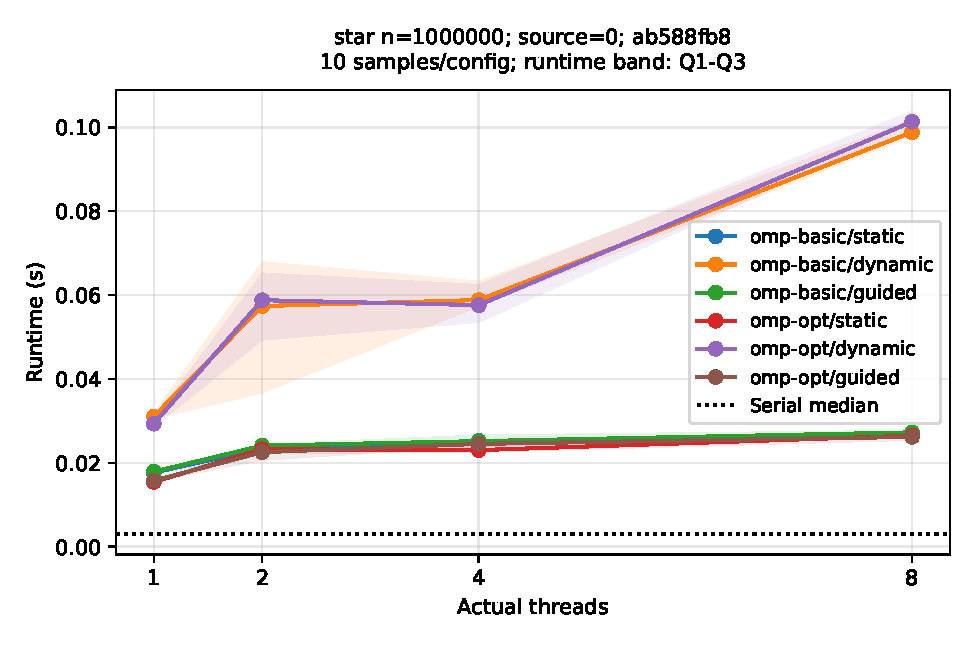
\includegraphics[width=.94\textwidth]{figures/experiment-20261112/star1000000-s0/median.pdf}
\caption[Star1000000: thời gian]{Star1000000, nguồn 0: median và dải IQR thời gian, 10 mẫu/cấu hình, commit ab588fb.}\label{fig:star-runtime}\end{figure}
\begin{figure}[p]\centering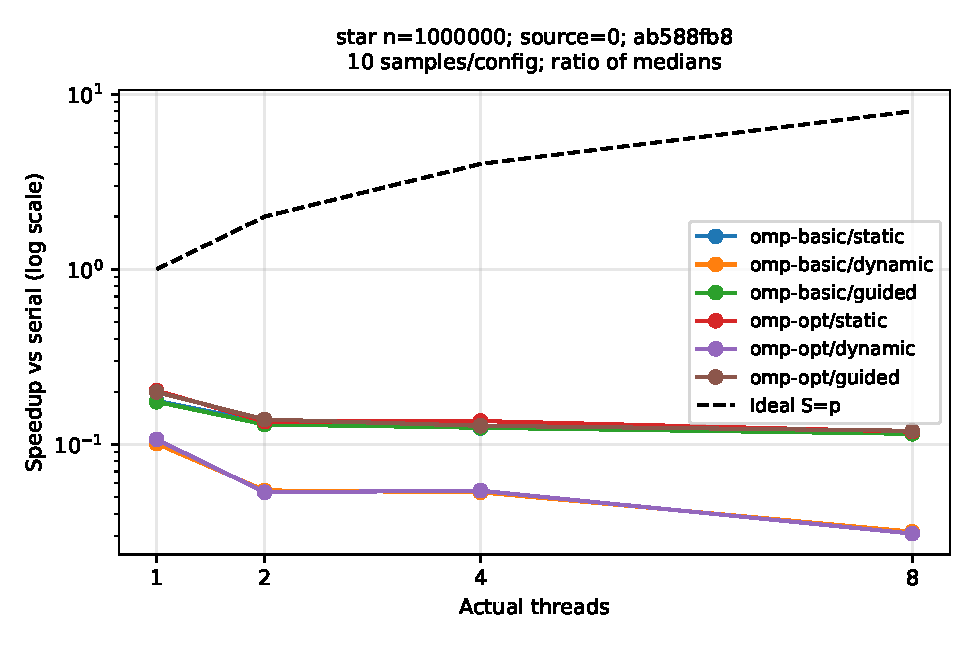
\includegraphics[width=.94\textwidth]{figures/experiment-20261112/star1000000-s0/speedup.pdf}
\caption[Star1000000: speedup]{Star1000000, nguồn 0: speedup so Serial và mốc $S=p$ trên trục log; mọi cấu hình dưới 1.}\label{fig:star-speedup}\end{figure}
\begin{figure}[p]\centering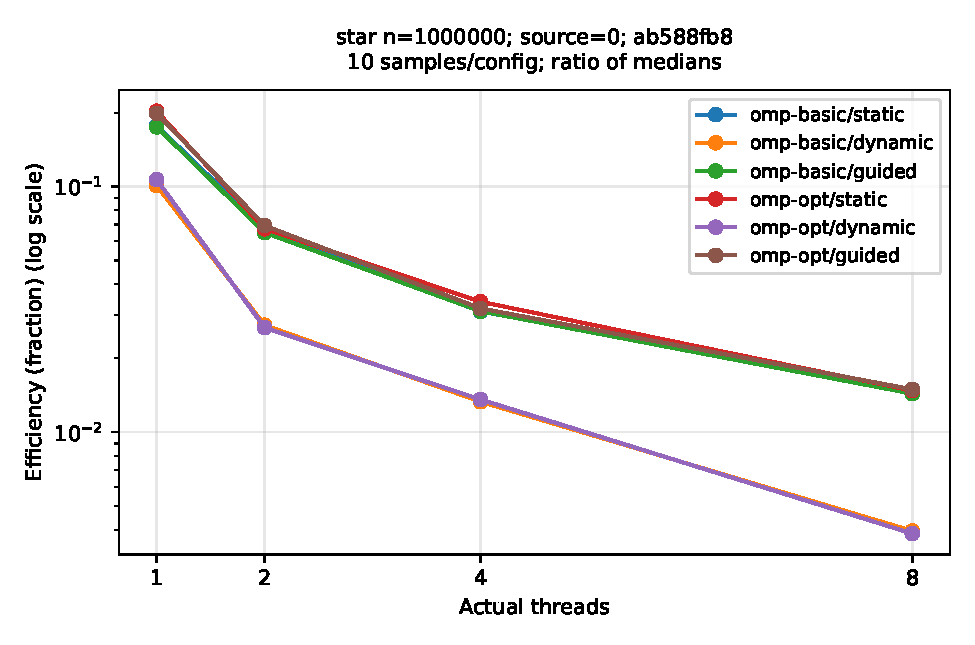
\includegraphics[width=.94\textwidth]{figures/experiment-20261112/star1000000-s0/efficiency.pdf}
\caption[Star1000000: efficiency]{Star1000000, nguồn 0: efficiency theo team thực, đơn vị phần số, không phải phần trăm.}\label{fig:star-efficiency}\end{figure}
\begin{figure}[p]\centering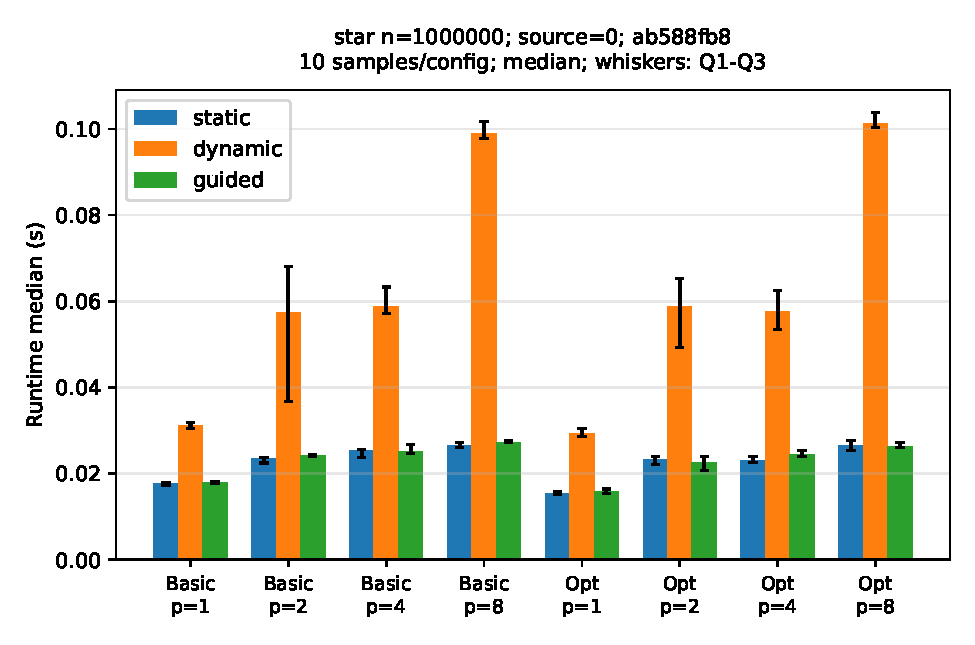
\includegraphics[width=.94\textwidth]{figures/experiment-20261112/star1000000-s0/scheduling.pdf}
\caption[Star1000000: scheduling]{Star1000000, nguồn 0: median và $Q_1$--$Q_3$ của ba schedule tại cùng team; dynamic chậm rõ ở nhiều luồng.}\label{fig:star-schedule}\end{figure}
\clearpage

\section{Grid: kích thước, số mức và nguồn}
Grid512 nguồn góc có Serial median 1,6942 ms, Basic8/static 112,6744 ms và Optimized 179,7294 ms. Speedup là 0,01504 và 0,009426; efficiency0,188\% và 0,118\%. Từ grid128 lên grid512, số đỉnh gấp16 và số mức từ góc gần gấp4; Basic8/static tăng30,5277 lên 112,6744 ms (3,69 lần), Serial tăng18,6 lần. Xu hướng phù hợp ảnh hưởng mạnh của số mức, nhưng chưa tách mọi nguyên nhân từ timer tổng.

Nguồn tâm131328 giảm khoảng cách lớn nhất từ 1022 xuống512. Basic8/static còn 62,3913 ms (giảm 44,6\%), Optimized 92,5461 ms (giảm 48,5\%). Serial lại tăng1,6942 lên 1,87115 ms, nên không có một xu hướng cho mọi thuật toán. Frontier rộng hơn và ít mức hơn có thể giải thích thay đổi OpenMP; thứ tự truy cập và điều kiện phiên chưa kiểm soát hoàn toàn.

Ở nguồn góc/actual 8, dynamic cho Basic143,5954 ms và Optimized 224,1793 ms, lớn hơn static 27,4\% và 24,7\%. Guided nằm giữa:127,8383 và 190,7862 ms. Optimized một luồng/static thấp hơn Basic (5,814 so 7,0432 ms), nhưng 8 luồng lại cao hơn 59,5\%. Giảm contention có thể đổi lấy prefix/copy/barrier; dữ liệu không ủng hộ lợi ích ổn định qua team. Xem Hình~\ref{fig:grid-runtime}--\ref{fig:grid-schedule}.

\begin{figure}[p]\centering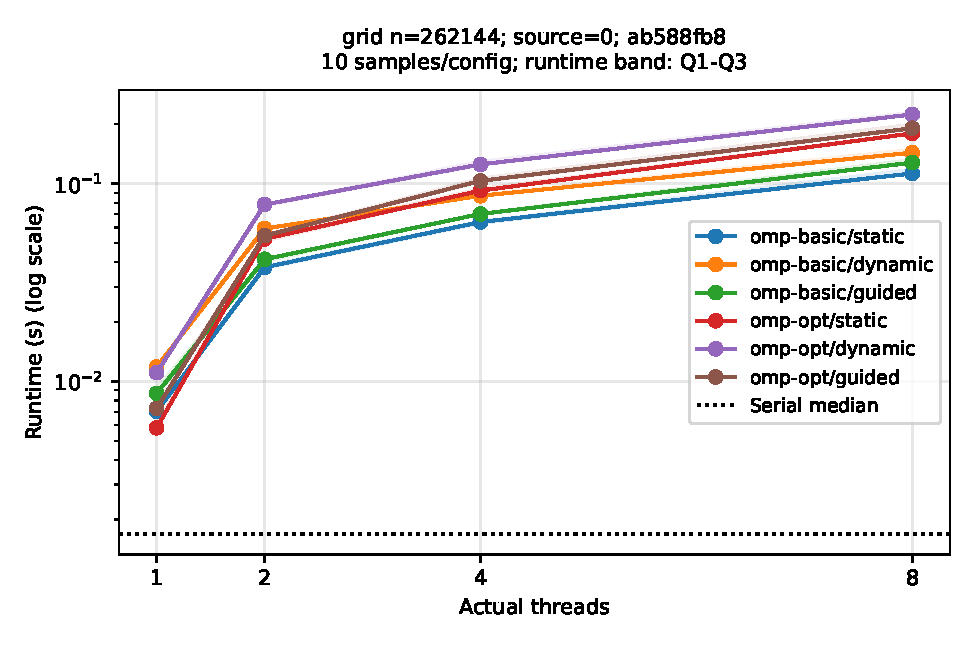
\includegraphics[width=.94\textwidth]{figures/experiment-20261112/grid512-s0/median.pdf}
\caption[Grid512: thời gian]{Grid512, nguồn 0: median và dải IQR thời gian; 10 mẫu/cấu hình, commit ab588fb.}\label{fig:grid-runtime}\end{figure}
\begin{figure}[p]\centering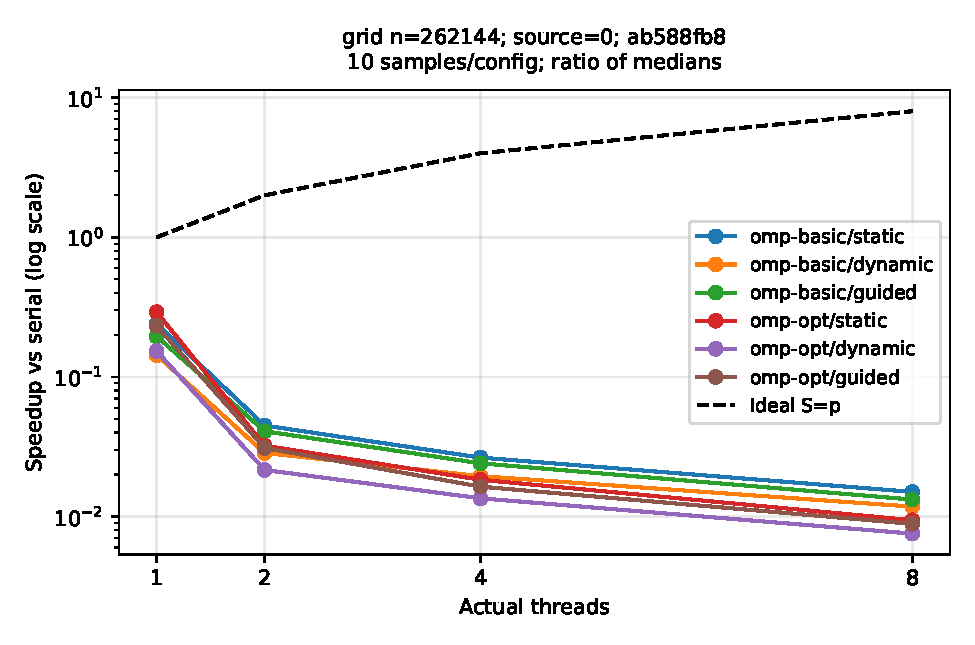
\includegraphics[width=.94\textwidth]{figures/experiment-20261112/grid512-s0/speedup.pdf}
\caption[Grid512: speedup]{Grid512, nguồn 0: speedup và mốc lý tưởng trên trục log. Optimized một luồng tốt nhất ma trận nhưng vẫn dưới 1.}\label{fig:grid-speedup}\end{figure}
\begin{figure}[p]\centering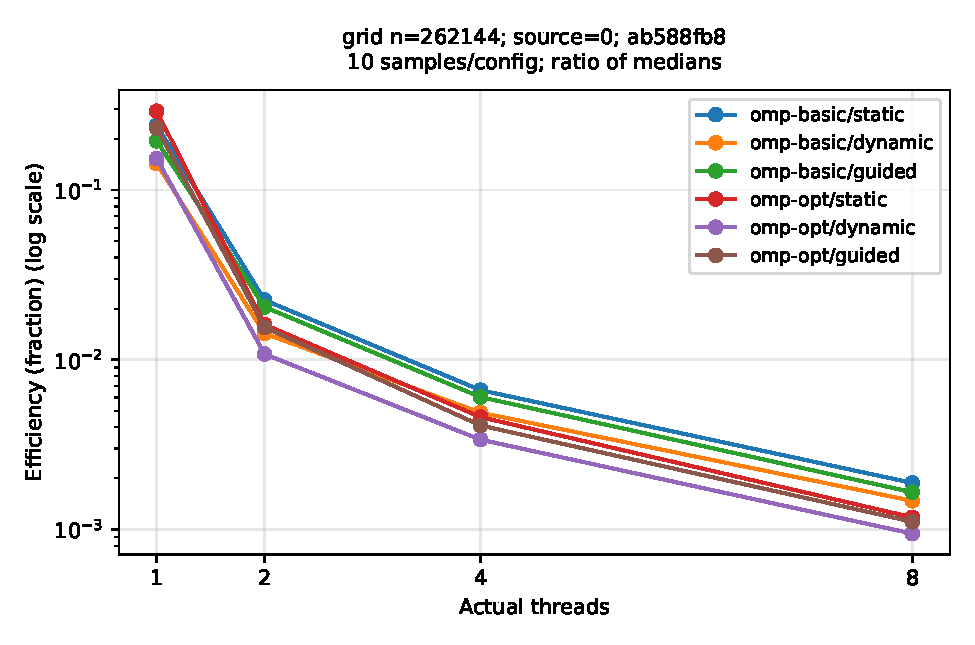
\includegraphics[width=.94\textwidth]{figures/experiment-20261112/grid512-s0/efficiency.pdf}
\caption[Grid512: efficiency]{Grid512, nguồn 0: efficiency theo actual team; không lấy requested threads thay team thực.}\label{fig:grid-efficiency}\end{figure}
\begin{figure}[p]\centering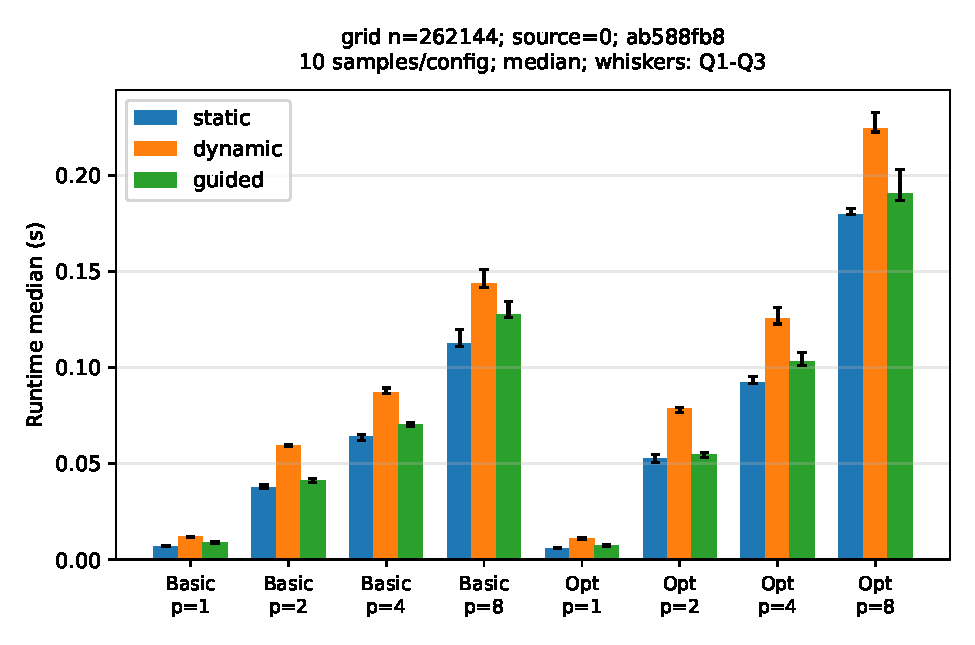
\includegraphics[width=.94\textwidth]{figures/experiment-20261112/grid512-s0/scheduling.pdf}
\caption[Grid512: scheduling]{Grid512, nguồn 0: median và $Q_1$--$Q_3$ của schedule tại cùng thuật toán/team.}\label{fig:grid-schedule}\end{figure}
\clearpage

\section{Đối chiếu câu hỏi nghiên cứu và độ tin cậy}
Correctness có oracle độc lập, full distance/CSR equality trong test và validation của 2475 lượt chạy; không quan sát lỗi trong phạm vi đã thử. Khả năng mở rộng không cho thấy tăng tốc: cả 216 cấu hình OpenMP có $S<1$, mọi cấu hình từ hai luồng có $C<1$. Hiệu năng thấp không làm kết quả khoảng cách trở thành sai, nhưng bác bỏ kỳ vọng tăng tốc cho phép đo này.

Optimized/scheduling phụ thuộc cấu hình: Optimized có median tốt hơn Basic ở một số cấu hình một/bốn luồng, song chậm hơn rõ trên path/grid ở 8 luồng; dynamic thường thêm chi phí trên star/grid. Không có bằng chứng một phiên bản/schedule luôn thắng. Các tỉ số mô tả median, chưa phải kiểm định thống kê khác biệt trung bình.

IQR/median lớn nhất khoảng 67,0\% ở Serial/star100000: median 0,2825 ms, min0,1870, max0,6137, $Q_1=0,1926$, $Q_3=0,381825$ ms. Mọi mẫu vẫn được giữ. Chênh lệch nhỏ hơn mức phân tán cần diễn giải thận trọng; QPC chỉ giải quyết lượng tử hóa1 ms, không loại tải nền hoặc scheduling Windows.

Dataset/nguồn chạy theo từng khối; shuffle chỉ trong khối nên còn sai lệch giữa thời điểm. Một máy, đồ thị có cấu trúc, team mới mỗi process, không affinity/profiling/nhiệt độ hoặc máy thứ hai là các giới hạn chính. Chưa có cơ sở suy luận về frontier rộng bất quy tắc hoặc BFS lặp với team đã nóng. sessions.json liên kết bảng/đồ thị với session, commit và manifest/raw hashes; summary.csv giữ đầy đủ thống kê để kiểm tra lại.
